\subsection{Verifica del funzionamento di un comparatore}

\begin{wrapfigure}[18]{r}{0.5\textwidth}
  \begin{center}
    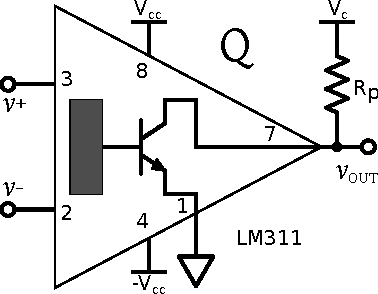
\includegraphics[width=0.280\textwidth]{../E04/latex/c_LM311.pdf}
  \end{center}
  \caption{Schema a collettore aperto dell'amplificatore operazionale LM311.}
  \label{cir4:open_collector}
\end{wrapfigure}

In questa prima parte dell'esperienza abbiamo verificato il funzionamento di un amplificatore operazionale LM311 come comparatore.
Questo amplificatore ha uno slew rate molto alto e lavora sull'ordine dei nanosecondi: rispetto agli $0.5$\si{\volt\per\micro\second} del $\mu$A741, lo slew rate particolarmente elevato permette di confrontare più velocemente i segnali.
Il funzionamento di questo integrato può essere semplificato, se valutato in configurazione di open loop, schematizzandone il funzionamento con un transistor BJT a collettore aperto, in il collettore del transistor rappresenta l'output dell'opamp e l'emettitore è collegato a comune (Figura \ref{cir4:open_collector}).
Se colleghiamo anche una resistenza $R$ fra una tensione arbitraria $V_C$, la funzione di output dell'operazionale diventa

\begin{equation}
V_{out} = \bigg \{
\begin{array}{rl}
V_C & \mathrm{se} \quad V_+ < V_- \\
0 & \mathrm{se} \quad V_+ > V_- \\
\end{array}
\label{eq4:comparatore}
\end{equation}

dove $V_+$ e $V_-$ sono rispettivamente le tensioni all'ingresso non invertente ed invertente. Utilizzando la schematizzazione con il transistor, è come considerare la condizione di quest'ultimo nella seguente maniera

%\begin{wrapfigure}[7]{l}{0.45\textwidth}
%  \begin{center}
%    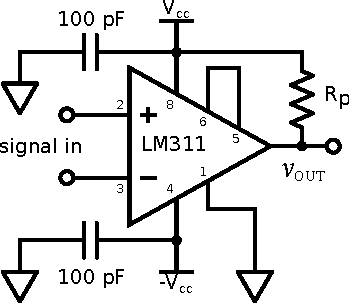
\includegraphics[width=0.30\textwidth]{../E04/latex/c_comparatore.pdf}
%  \end{center}
%  \caption{Schema completo del comparatore utilizzato. La resistenza $R_p=(9.98 \pm 0.01)$ \si{\kilo\ohm}, come consigliato sul datasheet.}
%  \label{cir4:comparatore}
%\end{wrapfigure}

\begin{equation}
Q : \bigg \{
\begin{array}{rl}
\mathrm{interdizione} & \mathrm{se} \quad V_+ < V_- \\
\mathrm{saturazione} & \mathrm{se} \quad V_+ > V_- \\
\end{array}
\label{eq4:comparatore_Q}
\end{equation}

da cui è facile mostrare che la tensione di uscita è proprio (\ref{eq4:comparatore}).

Infatti, quando Q è interdetto il generatore di tensione che fornisce $V_C$ non eroga corrente (l'impedenza dell'oscilloscopio è \SI{1}{\Mohm}) e non c'è caduta ai capi di $R$, dunque $V_{out}=V_C$; quando Q è in saturazione la tensione di uscita (tensione di collettore) si porta circa alla tensione di emettitore, dunque a zero\footnote{In realtà la tensione di uscita risulterà qualche centinaio di \si{\milli\volt} sopra lo $0$. Tale tensione serve a polarizzare il transistor affinché vada in saturazione oltre, ovviamente, alle cadute nelle altre parti della circuiteria interna dell'amplificatore.}. Si noti che la tensione di uscita può essere controllata solo grazie alla presenza della resistenza $R$.

Sfruttando questa funzione possiamo dunque confrontare la tensione in entrata su un ingresso con quella all'altro ingresso. Ad esempio, poniamo l'ingresso invertente ad una tensione di soglia $V_{ref}$: se vale la (\ref{eq4:comparatore}), ponendo un segnale in alternata sull'ingresso non invertente, l'operazionale restituirà una $V_{out}$ nulla se $V_{in}<V_{ref}$, altrimenti $V_C$. Valutiamo dunque il funzionamento del circuito ipotizzato, il cui schema circuitale è in Figura \ref{cir4:comparatore}, ponendo $V_{C}=5$\si{\volt}. Il grafico in Figura \ref{gr4:comparatore} mostra la tensione in entrata e in uscita.

\begin{figure}[ht]
 \centering
   {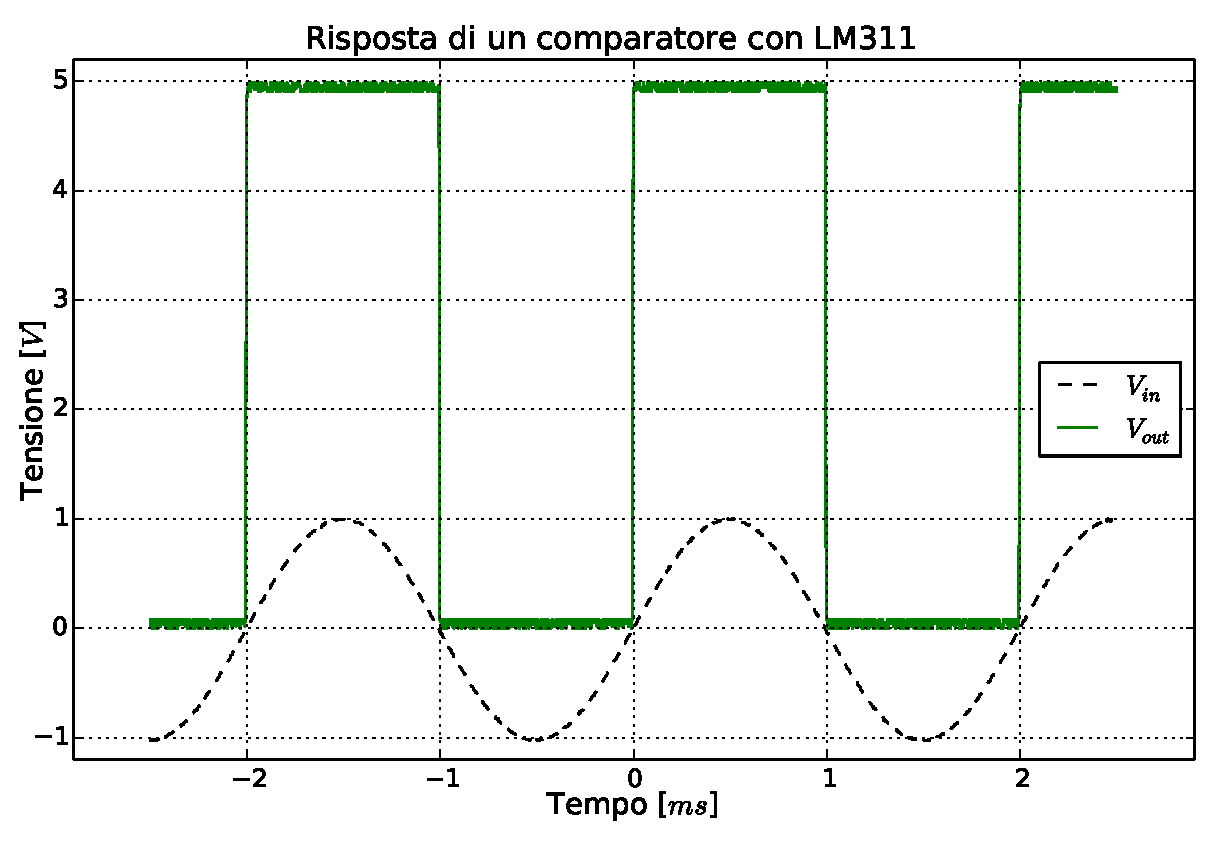
\includegraphics[width=14.5cm]{../E04/latex/comp.pdf}}
 \caption{Grafico della tensione in entrata (onda sinusoidale con $V_{pp}=2$ \si{\volt} e $f=500$\si{\hertz}, tratteggiata) e in uscita (verde) in funzione del tempo. Notiamo che l'uscita rispetta (\ref{eq4:comparatore}).}
 \label{gr4:comparatore}
\end{figure}